
\section{Introduction}

Imagine being a software development manager and hearing one of the worst possible pieces of news.  One of your top engineers, Dakota, just gave notice and is moving on to a new opportunity. You might be torn with mixed emotions. On one hand, you are excited because the new position provides a great career opportunity for someone you respect. On the other hand, you might worry about your project. How is the team going to manage this? You have been investing in this engineer. Your investment and all the engineer's accumulated knowledge and context about the code is walking out the door.  As one of your top performers, Dakota worked on the most important aspects, the trickiest parts, of your system. How long is it going to take others to ramp up on the code that Dakota owned? How is this loss in productivity going to affect future development? 

This paper introduces the theory of sustainable software development through collective code ownership as a solution to the problem of business sustainability for an ever changing workforce by enabling a team to repeatedly deliver complex systems and features and empowering a team so that any member of the team can work on any part of the system. The combination of practices actively works against creating knowledge silos and encourages the discoverability of code. The theory fosters cross-sharing knowledge and simplifying code to make it easy to maintain. As opposed to strong code ownership where one developer implements a complex feature, this theory requires that many developers shape the implementation as the baton of development is rotated through the team.

The theory emerged from Grounded Theory, an iterative research method. We collected empirical data from participant observations of an Extreme Programming project at Pivotal and interviews of Pivotal engineers, designers and product managers. As aspects of the theory emerged, we collected additional data to validate and saturate the theory.

In Extreme Programming, Kent Beck distills Collective Ownership practice into \quotes{Anyone on the team can improve any part of the system at any time.} He contrasts Collective Ownership against \quotes{no ownership} and \quotes{individual ownership.} He summarizes, \quotes{In Extreme Programming, everybody takes responsibility for the whole of the system. Not everyone knows every part equally well, although everyone knows something about every part. If a pair is working and they see an opportunity to improve the code, they go ahead and improve it if it makes their life easier.}  \cite{ExtremeProgramming2000} Later, Kent Beck renames Collective Ownership to Shared Code \cite{ExtremeProgramming2004}. 

Our initial core question was: \quotes{What is happening when it comes to software development at the studied organization?} When \quotes{collective code ownership} emerged as a core category, we collected additional sampling to identify which elements were required to enable collective code ownership and which situations would impact a programmer's sense of ownership. The observed project succeeded in spite of high team disruption. This observation leads us to new research questions: \quotes{How does Pivotal overcome team disruption in software development?}

In section \ref{RelatedWork}, we position the theory relative to existing literature. In section \ref{ResearchMethod}, we review how we employed Grounded Theory to derive a theory supported by empirical data. In section \ref{ResearchContext}, we present the research context, explaining both the company and project details. In section \ref{Theory}, we describe the theory and how its principles, policies, and practices work together to achieve the observed results. In section \ref{Transitioning}, we examine nuanced issues of transitioning to collective code ownership. In section \ref{TheoryEvaluation}, we evaluate the theory using established criteria for evaluating a grounded theory. In the last sections, we examine threats to research validity, examine future research, and conclude the research.


\section{Related Work}
\label{RelatedWork}
In Extreme Programming \cite{ExtremeProgramming2004} Kent Beck describes a set of interdependent practices that manage feature development (much like Scrum \cite{Scrum}), as well as technical practices that facilitate a collaborative team environment.  Extreme Programming comprises 13 primary practices and 11 corollary practices. Many of the practices are dependent on each other.  {In Extreme Programming, everybody takes responsibility for the whole of the system. Not everyone knows every part equally well, although everyone knows something about every part. If a pair is working and they see an opportunity to improve the code, they go ahead and improve it if it makes their life easier}  \cite{ExtremeProgramming2000}.



The concepts of Lottery Number, Bus Count, Lorry Number, or Truck Number remind management about the effects of disruptive events for a team. Truck Number is, \quotes{The size of the smallest set of people in a project such that, if all of them got hit by a truck, the project would be in trouble.} \cite{WikiTruckNumber}. 

In 1994, James Coplien mentions Truck Number as a risk to his Solo Virtuoso pattern of using only one talented developer to create a software system \cite{Coplien1994}. 

In 2008, Kailash Awati suggests three strategies for increasing Bus Count: reducing complexity, documentation, and cross-training \cite{AwatiBusFactor}. All three strategies are found in Extreme Programming if documentation morphs into easily discoverable, intention revealing code. Little academic research has examined this topic. 

%\subsection{Code ownership}
%In 2006, Martin Fowler defines collective code ownership similarly to Kent Beck \cite{FowlerCodeOwnership} as a contrasting team position to \quotes{strong code ownership} where each file is owned by one person and `\quotes{weak code ownership} where developers can change files but an owner keeps an eye on the file since they are responsible for it. 

%Collective Code Ownership requires more than a team saying \quotes{everyone can modify anything}. Instead, we are interested in how much the team feels that they collectively own the code. We shift from a policy statement to a \quotes{sense of collective code ownership.} We define \quotes{sense of collective code ownership} as the degree to which individual members of the team feel collective ownership.  

%This work builds upon the significant accomplishments of Extreme Programming and refines it with other practices. For example, in Extreme Programming, it is possible for a developer to work on the same track of work creating a knowledge silo. This is an undesirable property for collective code ownership. This work introduces an explicit rotation practice.

This research shows that one way to achieve collective code ownership is to enact all of the practices of Sustainable Software Development.

%Todo: This paper looks at ownership in organizations \cite{PierceOwnershipInOrganizations}
\section{Research Method: Grounded Theory}
\label{ResearchMethod}

We followed Grounded Theory, \cite{Charmaz} which provides an iterative approach to data collection, data coding, and analysis resulting in an emergent theory. We selected Charmaz' constructivist approach to Grounded Theory that situates ...
The two primary data sources were field notes collected during continuous participant observations of a 7.5 month project and interviews with Pivotal software engineers, designers, and product managers. Interviews were recorded, transcribed, coded, and analyzed using constant comparison. 

Grounded Theory immerses the researcher within the context of the research subject from the point of view of the participants. As the research progresses, Grounded Theory allows the researcher to \quotes{incrementally direct the data collection and theoretical ideas.} The theory provides a starting place for inquiry, not a specific goal known at the beginning of the research. As we interact with the data, the data influence how we progress and alter the research direction. When starting a grounded theory research study, the core question is, \quotes{What is happening here?}' (Glaser, 1978) \cite{GlaserTheoreticalSensitivity}. Our initial core question was, \quotes{What is happening at Pivotal when it comes to software development?}

\subsection{Participants}
The primary researcher interviewed 21 engineers, product managers, and designers who had experience with Pivotal's software development process. Designers identify user needs through user interviews; create and validate user experience with mockups; determine the visual design of a product; and support engineering during implementation. Product managers are responsible for identifying and prioritizing features, converting features into stories, and prioritizing stories in a backlog.  Participants were not paid for their time. 
\subsection{Data Collection}
The primary researcher relied on \quotes{intensive interviews} which Charmaz summarizes as \quotes{open-ended yet directed, shaped yet emergent, and paced yet unrestricted} \cite{Charmaz}. The technique relies on open-ended questions. The purpose is for the researcher to enter into the participant's personal perspective within the context of the research question. The interviewer needs to abandon assumptions and their own personal presumptions to understand and explore the interviewee's perspective. Charmaz \cite{Charmaz} contrasts intensive interviews from informational interviews which endeavor to collect accurate `facts' and investigative interviews that attempt to reveal hidden intentions or expose practices and policies. 
 
The interviews were open-ended explorations starting with the question, \quotes{Please draw on this sheet of paper, your view of Pivotal's software development process.} The interviewer specifically didn't force initial topics and merely followed the path of the interviewee. 

While exploring new emergent core categories, whenever possible, the researcher initiated subsequent interviews with a goal of not forcing the issue. For example, \quotes{Please draw your feelings about the code} often resulted in conversations about code ownership. 

After completing the interview, it was transcribed into a Word document with timecode stamps for each segment.

In addition to collecting data from interviews, the primary researcher collected field notes while working as a engineer on the project described in section \ref{ExampleInAction}. The field notes comprised multiple paragraph entries recorded several times a week, collected over a six month period. The field notes described individual and collective actions, captured what participants defined as interesting or problematic, and included anecdotes and observations. 
\subsection{Data Analysis}
The primary researcher followed line-by-line coding as recommended by Charmaz \cite{Charmaz}. The line-by-line coding helped the researcher slow down and examine for nuanced interactions in the data. Based upon Charmaz's advice, the primary researcher adopted a coding scheme that was simple, direct, analytic, and spontaneous.  

After the initial coding, another researcher reviewed the initial codes while reading the transcripts and listening to the audio recording. During a weekly research collaboration meeting, any concerns were discussed and addressed. During these meetings, we recorded and transcribed into grounded theory memos any discussions about analysis or understanding the codes. Recording the sessions mitigated Glazer's concerns about missing possible memos or insights that are verbally discussed \cite{GlaserTheoreticalSensitivity}.

As data was collected and coded, the researcher placed the codes into a spreadsheet. The researcher followed constant comparison which resulted in focused codes.  The researcher compared new codes to existing codes for emergence of new categories. Only ideas shared by multiple interviewees earned their way into focused codes and subsequent analysis. The primary researcher periodically audited each category by comparing the codes to each other and verifying the cohesion of the category. For complex categories, the codes were printed onto index cards, then the cards were arranged and re-arranged until logical categories emerged.  The researcher captured the analysis of codes, examinations of theoretical plausibility, and insights in memos. 

Analytical work revealed emergent categories which were then explored deeper in subsequent interviews.  Once emergent themes arrived, coding in later parts of the research focused around the emergent themes. The focused coding phase allowed the primary researcher to ``sort, synthesize, integrate, and organize large amounts of data."

As theoretical codes emerged, the researcher altered data collection for saturating core categories. When collective code ownership emerged as a core category, the researcher collected additional sampling in order to identify which situations would increase or decrease a programmer's sense of ownership and which practices were required to enable collective code ownership.

\section{Research Context}
\label{ResearchContext}
\subsection{Organizational Context: Pivotal}
Pivotal is a large American software company, which provides solutions for cloud-based computing, big data, and agile development. For example, Pivotal Cloud Foundry is an open source Platform as a Service either on-premise or hosted in the cloud, while Pivotal Big Data Suite stores and analyzes multiple large data sets using Hadoop, Hawq, and Green Plum. Pivotal Labs meanwhile provides agile developers and designers for startups and enterprise companies to transform their software development process. Pivotal Labs has offices in Palo Alto, Berlin, Boston, Boulder, Chicago, Denver, Dublin, London, Los Angeles, New York, San Francisco, Seattle, Sydney, Tokyo, Toronto, and Washington District of Columbia. At the start of this research 18 months ago, Pivotal practiced this way of working in nine offices. At the time of writing this paper, Pivotal has 16 offices. 

Pivotal Lab's mission is not only to deliver highly-crafted software products, but also to provide a transformative experience for their clients' engineering cultures. To change a developer's way of working, Pivotal combines the client's software engineers with Pivotal's engineers at a Pivotal office where they can experience Extreme Programming in an environment conducive to agile development. This experience is similar to the creation of the NUMMI plant where General Motors sent workers to Japan to learn Toyota's Production System \cite{Nummi}. For startups, Pivotal engineers might be the first to work on the project. For enterprise clients, Pivotal provides additional engineering resources to accomplish new business goals. Sometimes, Pivotal helps transform engineering cultures when they no longer routinely deliver code.  

Common team sizes are six developers with a designer and a product manager. In the Palo Alto office, the number of developers on a project currently ranges from 2 to 28. Larger projects are decomposed into smaller coordinating teams with one product manager per team and one or two designers per team. 

Commonly utilized technologies include Angular, Android, backbone, iOS, Java, Rails, React, and Spring and are often deployed onto Pivotal's Cloud Foundry. 

Pivotal Labs has followed Extreme Programming \cite{ExtremeProgramming2004} since the late 1990's. While each team autonomously decides what is best for each project, the company culture strongly suggests following all of the core practices of Extreme Programming, including Pair Programming; Test Driven Development; Weekly Retrospectives; Daily Stand-ups; Prioritized Backlog; Whole Team ownership of the project and code base; and Kanban's notion of work flowing through people.

In addition to the intensive interviews, the primary researcher asked all of the software engineers, designers, and product managers at the Palo Alto office the question, \quotes{Given all of the values, principles, and practices of Pivotal, what do you think is the heart of the matter, what is core to all we do?} Table \ref{CorePractice} includes the various answers. The diversity of answers shows little consensus around Pivotal's core. 

\begin{table}[t]
\renewcommand{\arraystretch}{1.3}
\centering
\caption{Answers to \quotes{What is core to all we do?} show no common understanding of what is core}
\label{CorePractice}
\begin{tabular}{|p{3.10in}|}
\hline
\quotes{empathy} \\ \hline
\quotes{teamwork} \\ \hline
\quotes{communication} \\ \hline
\quotes{doing things the right way} \\ \hline
\quotes{constant communication} \\ \hline
\quotes{collaboration} \\ \hline
\quotes{pairing, TDD} \\ \hline
\quotes{TDD, agile planning, pair programming} \\ \hline
\quotes{feedback, fast feedback loop} \\ \hline
\quotes{kindness, no matter what you do, if you hurt people, that's not good. Software is built by humans. Act human} \\ \hline
\quotes{user research and feedback} \\ \hline
\quotes{delivery of value to the customer} \\ \hline
\quotes{keeping clients paying us means that I have a job. Pairing has a very real impact in attracting clients. TDD has large impact on code quality. Once I leave pivotal, TDD is what I will take to my next job} \\ \hline
\quotes{doing the right thing} \\ \hline
\quotes{iteration practices drive our other practices. We do lean design. Build Measure Learn} \\ \hline
\quotes{short feedback loops both at the project level and personal level when people giving me feedback} \\ \hline
\quotes{empathy} \\ \hline
\quotes{pairing, testing} \\ \hline
\quotes{self reflection and  team retros} \\ \hline
\quotes{doing the right thing} \\ \hline
\quotes{enabling companies to build great software} \\ \hline
\quotes{guaranteed repeatable success} \\ \hline
\quotes{kindness, feedback loops, bias towards action} \\
\hline
\end{tabular}
\end{table}

\subsection{Project Context: Project Quattuor}
\label{ExampleInAction}
Imagine that you are staffing a 10 person project for 8.5 months. From experience, you know that over that period of time some people might come and go. What is the maximum number of people you would be comfortable working on that project so that the team is productive and achieves a successful outcome?  

Project Quattuor is a 43 week project. The initial 4 weeks are called Design and Framing, where user needs are gathered by designers through user interviews, product managers define the features for the initial release based on those needs, designers create an initial interaction design and validate their mock-ups with users, and engineers mitigate technology risks. Design and Framing is followed by code implementation, resulting in two releases to the Apple store and Google play store.

\begin{figure*}[t]
\centering
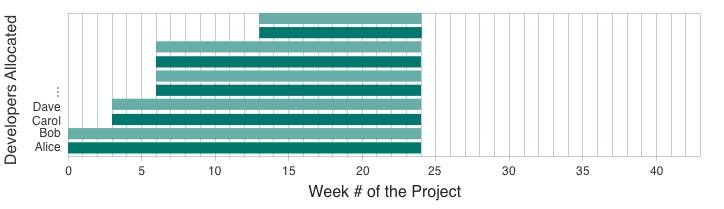
\includegraphics[width=7.1in]{OriginalDeveloperStaffingV2.jpg}
\caption{Planned Developer Staffing}
\label{PlannedDeveloperStaffing}
\end{figure*}

The entire 35-person project consisted of an iOS team of 10 engineers, an android team of 10 engineers, and a Java back-end team of 8 engineers with the support of 2 to 4 designers and 3 product managers. For the purpose of this discussion, we will focus on the iOS team. 

The first iOS release to the Apple store occurred on week 23. Give the success of the project, the client extended the engagement for a second iOS release that occurred on week 43. 

On a typical project, the project is a stable team organically grown. Figure \ref{PlannedDeveloperStaffing} shows the staffing plan at the start of Project Quattuor. Two developers started the project with more developers rolling on as there were more tracks of work. The top diagram shows when individual developers start and stop on the project. The bottom diagram shows the total number of developers allocated to the project at any given week. 

On this project, developers were routinely rotated off and replaced for a variety of reasons, including being promoted to management, taking medical leave, leaving the company, transferring to a different office, transferring to another project, and taking vacations. 

The client wanted to maximize feature development regardless of cost. On a typical project, if an engineer goes on vacation, the team remains the same and is slightly less productive. On this project, someone took that person's place while the person was gone. This resulted in many engineers rolling on and off the project. A total of 22 people worked on the ten-person project. The ongoing rotation of team members likely undermined the team's sense of identity \cite{TuckmanModel}.

\begin{figure*}[t]
\centering
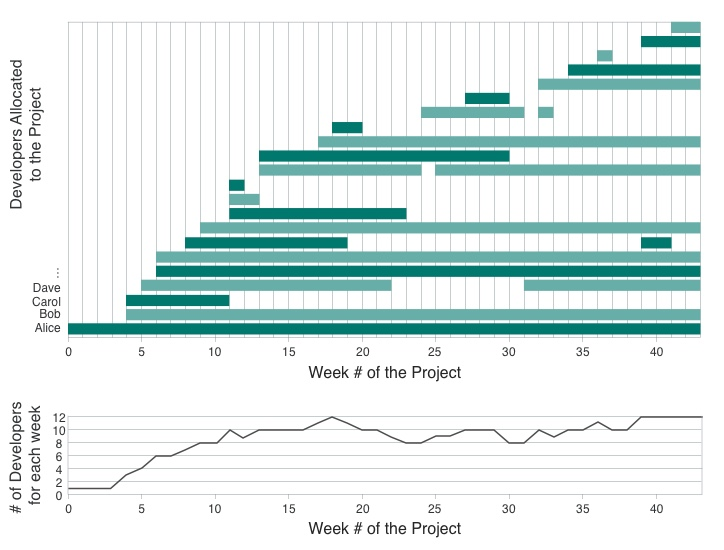
\includegraphics[width=7.1in]{DeveloperStaffing.jpg}
\caption{Actual Developer Staffing}
\label{DeveloperStaffing}
\end{figure*}

Figure \ref{DeveloperStaffing} shows the actual project staffing.  The top diagram shows that there were five developers who were on the project for most of its duration, that 22 people actually worked on the project, and that the maximum team size was 12 developers working together at the same time.

The bottom diagram shows the total number of developers allocated to the project at any given week. There is a steady ramp up from week 5 to week 12. The average number of developers assigned to the team is 9.8 and the maximum team size was 12 developers.

The project experienced many challenges, including the unstable team, not having access to production back-end systems or expensive dependent physical components, and cultural differences between Pivotal and the client's deployment organization. Yet the team successfully completed the project. The client was delighted, even claiming with the first release that the team had delivered a multiple year project in 5 months. 

Conventional wisdom says that team churn is disruptive for a team and should be avoided. Yet, Project Quattuor succeeded despite high team churn. This observation leads us to our first research question: \quotes{How does Pivotal overcome the team churn challenge in software development?}

\section{Theory of Sustainable Software Development}
\label{Theory}

A theory of Sustainable Software Development emerged from the grounded theory research. Sustainable Software Development is characterized by a positive attitude towards team disruption, together with a collection of synergistic policies and practices encouraging knowledge sharing and continuity, as well as caring about code quality. Knowledge sharing and continuity enables the business entity to overcome disruptions, such as vacations, rotation of team members, churn, and growing team size. Engineering teams repeatedly deliver software features, even when disrupted, while working with complex systems or legacy code bases. This theory results in throughput sustainability by establishing a software development culture where each developer is both empowered and enabled to modify any portion of the code base. As a result, each engineer becomes replaceable, which ironically makes the team irreplaceable as it is performant and can handle challenging situations. The theory answers the following research question:

Research Question 1: How does Pivotal overcome team disruption in software development?

Pivotal overcomes the challenge of team disruption through a set of principles, policies, and practices.

\subsection{Principles}

\begin{table}[]
\renewcommand{\arraystretch}{1.5}
\centering
\caption{Underlying Principles of Sustainable Software Development}
\label{TheoryPrinciples}
\begin{tabular}{l}
\hline
Keeping a Positive Attitude Toward Team Disruption \\
Encouraging Knowledge Sharing and Continuity \\
Caring about Code Quality \\
\hline
\end{tabular}
\end{table*}

\subsubsection{Keeping a Positive Attitude Toward Team Disruption}
Conventional wisdom says that team disruption should be avoided. Yet, team disruption is a reality in the industry, as exemplified by Project Quattuor where only four of twenty-two developers worked on the project for from beginning to end (see Figure \ref{DeveloperStaffing}.) However, the observed organization keeps a positive attitude towards disruption, transforming a challenge into an opportunity and hence demonstrating a remarkable business agility. Team members rolling off the project were replaced as needed. New members rolling onto the project were viewed as an opportunity to improve the current code base by providing a fresh, new perspective. When a new team member did not understand the code base, he or she revealed issues with code discoverability. New team members often questioned the team's assumptions and challenged cargo culting. 

The first underlying principle of Sustainable Software Development is keeping an open and positive attitude towards team disruption, transforming a challenge into an opportunity to improve code quality.

\subsubsection{Encouraging Knowledge Sharing and Continuity}
Despite the fresh perspectives added by new team members, team disruption could potentially result in significant knowledge loss for the organization. A set of policies and practices aiming at encouraging knowledge sharing and continuity mitigate this risk. These policies are Collective Code Ownership and Shared Schedule, while the practices are Continuous Pair Programming, Overlapping Pair Rotation, and Knowledge Pollination. Refer to the following sections for more on these policies and practices. 

The second underlying principle of Sustainable Software Development is encouraging knowledge sharing and continuity, enabling the knowledge to spread from one developer to the next, and eventually reach the entire team. Knowledge sharing and continuity make the team more resistant to disruption. 

\subsubsection{Caring about Code Quality}

Enabling knowledge sharing and continuity does not guarantee sustainable development if the team starts incurring technical debt  \cite{McConnellTechnicalDebt}. A set of policy and practices aimed at taking good care of the code itself mitigated this risk. The policy is Avoid Technical Debt, while the practices are Test Driven Development / Behavior Driven Development and Continuous Refactoring. Refer to the following sections for more on these policy and practices.

The third underlying principle of Sustainable Software Development is caring about code quality, hence avoiding technical debt and enabling sustainable team productivity.

Table \ref{TheoryPrinciples} summarizes these principles. Table \ref{TheoryPractices}  summarizes a set of policies and practices that implement the principles which are recorded in the following sections. For each practice, we present how it is used at Pivotal, and discuss anti-patterns and potential alternatives. We provide deeper descriptions for practices rarely documented in the literature.
\subsection{Policies}

\begin{table*}[]
\renewcommand{\arraystretch}{1.5}
\centering
\caption{Theory of Sustainable Software Development: Policies and Practices}
\label{TheoryPractices}
\begin{tabular}{l|l|l}
\hline
\multicolumn{3}{c}{Sustainable Software Development}                               \\
\hline
Policies                  & Removing Knowledge Silos Practices & Caretaking the Code Practices         \\
$\bullet$ Collective Code Ownership & $\bullet$ Pair Programming         & $\bullet$  TDD / BDD                   \\
$\bullet$ Shared Schedule           & $\bullet$ Overlapping Pair Rotation & $\bullet$ Continuous Refactoring      \\
$\bullet$ Avoid Technical Debt      & $\bullet$  Knowledge Pollination    & Supported by Live on Master \\ 
\hline
\end{tabular}
\end{table*}

\subsubsection{Collective Code Ownership}
Collective code ownership conveys that any developer on the team can improve any part of the system at any time \cite{ExtremeProgramming2004}. Everyone is responsible for the the whole system. 

At Pivotal, every developer is empowered to work on any part of the system and is encouraged to refactor any code section to improve its quality as needed, especially when code discoverability and readability is an issue.

An organization saying, \quotes{Anyone can modify any piece the code} is not sufficient to achieve the desired result of collective code ownership. Achieving collective code ownership requires a set of enabling practices. These enabling practices aim at removing knowledge silos and taking good care of the code, as described in the following sections.

Removing collective code ownership makes sustainable software development challenging. Every line of code written via strong ownership creates a knowledge silo. Code reviews are a mitigation strategy with an asynchronous delay. When the delay is too long, merging code onto the master becomes problematic, which then places pressure to avoid Continuous Refactoring.  

\subsubsection{Shared Schedule}

Shared Schedule signifies that all project team members share the same work schedule. 

For instance, at the Pivotal Palo Alto office, team members start working at 9:00 in the morning and leave at 5:00 in the evening, five days a week. This is done without management coercion; each team member agreed to this fixed schedule to achieve the benefits of Sustainable Software Development. When shared schedule is the normative, then flexibility is possible for exceptions. For instance, seeing the doctor during the day is fine since it is important to take care of oneself.

Pivotal prefers for all team members to be colocated as it promotes synchronous and osmotic communication. As an exception, Project Quattuor was a two office project with half the team members in Palo Alto and half the team members in San Francisco. The team utilized remote pairing each day for Knowledge Pollination. Future research could explore whether Sustained Software Development works for a distributed team with a Shared Schedule.

Flexible work hours potentially jeopardizes the Pair Programming, Overlapping Pair Rotation, and Knowledge Pollination practices. 

A team with flexible work hours might find it difficult to pair program on all stories (as described in the Pair Programming practice). A team member consistently soloing from 8:00am to 10:00am might be building knowledge silos. Pivotal experimented with pairing when developers arrived, but this meant that developers arriving early were making decisions for the team members who arrived later, hence loosing some benefits of pair programming. 

When developers arrive whenever they feel like it, rotating pairs (as described under the Overlapping Pair Rotation practice) becomes awkward, as there is no longer a natural time to rotate pairs. With Shared Schedule, the team forms new pairs at the beginning of the day. The evening becomes a natural interruption to the continuous software development workflow. Trying to schedule a time midday to rotate feels artificial. Even if the team says they will rotate later in the day, once pairs get into their stories and form context on what needs to be done, they typically forget about repairing until it is time to go home.

A possible mitigation strategy would be to adopt core work hours. Individuals would solo on simple clean-up chores outside of core hours, and switch to pair programming for feature development when the whole team is in the office. 

\subsubsection{Avoid Technical Debt}

Technical Debt refers to delaying needed technical work when technical shortcuts are taken, usually in pursuit of calendar-driven software schedules \cite{McConnellTechnicalDebt}.  Continuous Refactoring (as described under the Continuous Refactoring practice) is one way to prevent technical debt from accumulating. When a team employs continuous refactoring, the team refines a code base towards simple design, intention revealing code, and discoverable code. 

At Pivotal, when the team implements a feature, the team desires to build it well. A pair tends to create well-crafted code by avoiding shortcuts and short-term fixes. Even with changing features or a changing product vision, the team strives to have well-engineered code. The team codes for the \quotes{present} by building the simplest solution for the current story. The team eschews over-engineering for potential future features. The team avoids technical debt by building the best solution for the moment at hand.  

When a team is pressured to finish work by a deadline, they might be tempted to focus on feature delivery, take on technical debt, and stop refactoring. When a team delays refactoring and takes on technical debt, the code becomes harder to work with, which in turn makes it harder for developers to rotate onto that part of the code base. The pair making the decision to skip refactoring is causing future pain for the next pair to work with this part of the code. 

On Project Quattuor, the product manager suggested that the team deliver more stories at the cost of technical debt to make a release date. Some team members followed this suggestion, skipped the refactoring step, and introduced harder to maintain code. This decision made it difficult for pairs to rotate onto parts of the code. Immediately after the release, the team spent several weeks refactoring the code to pay down the debt and be able to consistently deliver new features again.  
\subsection{Practices for Removing Knowledge Silos}
This section presents practices encouraging knowledge sharing and continuity, enabling the knowledge to spread from one developer to the next, and eventually reach the entire team, as illustrated in Figure 3.

\begin{figure}[t]
\centering
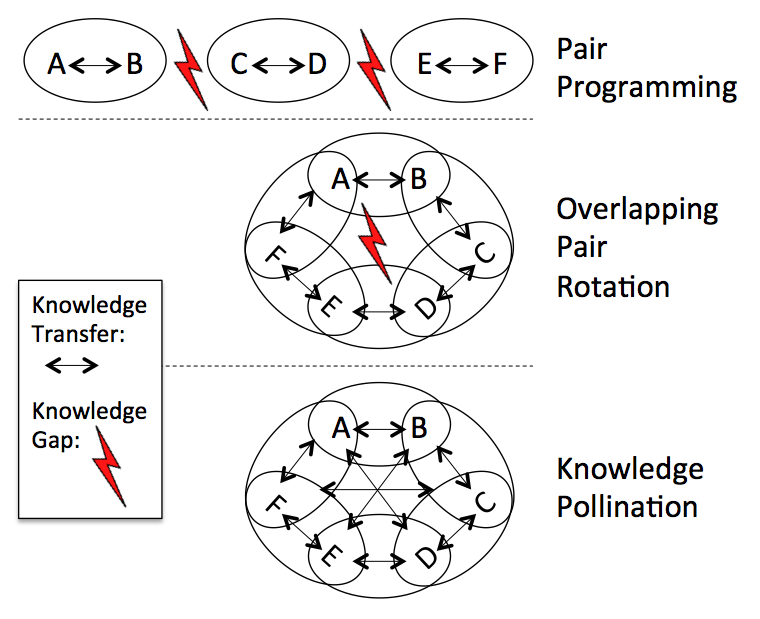
\includegraphics[width=3.4in]{KnowledgeSharingLevels.png}
\caption{Three Levels of Knowledge Sharing}
\label{KnowledgeSharing}
\end{figure}

\subsubsection{Pair Programming}
%what
\textbf{Description:} Pair programming is characterized by two developers collaborating to write software together. 

%why
\textbf{Purpose:} When two developers work together, they are likely to bring more knowledge, and generate more diverse solutions compared to a solo developer. Having two pairs of eyes increases the potential of catching defects. When two developers work together, knowledge spreads from one developer to the next, as illustrated in Figure 3. Overall, pair programming has the potential to reduce knowledge silos and improve code quality.

%at pivotal
\textbf{At pivotal:} Pairing happens with two monitors, two keyboards, two mice, and one computer. Developers always work in pairs, unless exceptional circumstances arise. For instance, solo programming occurs when one developer is out of the office part of the day (e.g. at home to let a plumber in, or at the doctor's office) or out of the office the whole day (e.g. out sick) or involved in another business activity for a few hours (e.g. interviewing candidates, scoping a new project). When solo programming, developers take low risk chores, refactorings, or stories. With any sizable project, there usually is something the team has been meaning to do that one person can safely do and report back to the team on its completion.  

%removing
\textbf{Anti-pattern:} Removing this practice results in solo programming where there is a clear owner for the code written. This would increase individual ownership and start creating knowledge silos. 

%alternatives
\textbf{Alternatives:}  In solo programming, to remove silos, developers could take the stories for the part of the code they know least about. Assigning stories to developers who have the least understanding of the code could be a hard sell to management as it slows productivity down (at least initially). Bird's study \cite{BirdDontTouchMyCode} suggests that this appoach would introduce more defects. 

\subsubsection{Overlapping Pair Rotation}
%what
\textbf{Description:} Overlapping Pair Rotation happens when there is a daily rotation of the pair working on a track of work, together with one team member remaining on the track of work for knowledge continuity as illustrated in Figure 3. For a track of work, we want one developer to roll off and another developer to roll on.  We do not want one developer working on the same track for three days in a row. Likewise, if any story lasts longer than a day, then one developer needs to rotate. Evenings provide a natural rhythm to rotating work. 

%why
\textbf{Purpose:} Rotation of developers helps prevent knowledge silos from forming. The goal is to prevent the situation where Jackie must be on the story since Jackie is the only person who understands how that part of the system works. Instead, the entire team should be able to modify the code. \quotes{Marion really knows the Apple watch code base, we need her on that story, or Shea knows the ins-and-outs of the siteminder integration, we need him to work on this} are signs that knowledge silos have emerged. 

%at pivotal
\textbf{At pivotal:} Whenever a knowledge silo begins to emerge, the team actively fights against it and tries to spread that knowledge around through pair rotation. 

Most teams rotate based on who has paired with whom and try to pair with the person they \quotes{least recently paired with} (basically an LRU strategy). This strategy does not clearly articulate the need for knowledge transfer. Developers ask to be rotated back onto a track that they enjoy working on without realizing the potential cost to the team. 

Some teams are experimenting with rotating the last person to work on that track. The goal of the developer who will leave the track tomorrow is to empower the new pivot to own the track the next day. When the rotation happens the next day, the second pivot is asked, \quotes{Was enough context shared with you?} If the answer is no, then the pair continues longer. This provides a feedback loop on how well the team is transferring knowledge.  

%removing
\textbf{Anti-pattern:} Removing this practice means that developers can work on the same part of the code base for extended periods of time, developing individual code ownership and knowledge silos. One of the interviewees worked at Xtreme Labs (a company that follows Extreme Programming and was acquired by Pivotal in 2013) where developers could be paired for more than a month working on only one part of the system. This lack of pair rotation led to building deep knowledge silos. 

Ideally developers work on the next, non-blocked story at the top of the backlog. When developers start skipping down the backlog, it can be an indication that they might not have enough context to work on any story. On Project Quattro, there was a knowledge silo with a complex bug related to an obsolete technology that only a handful of people understood. Often developers would skip over stories and bugs related to that technology. At one point, the product manager reminded the team to keep \quotes{working from the top of backlog.}

Sometimes a developer would want to see a story through to completion. Maybe he or she loves the technology or the feature. In these situations, the team needs to be careful about forming knowledge silos and creating a sense of personal ownership.

%alternatives
\textbf{Alternatives:} Team members that build a knowledge silo can share what they learned through a demo, code walk through, or a team huddle. This helps a team share knowledge, but is less effective than working with the code for eight hours. 

\subsubsection{Knowledge Pollination}
%what
\textbf{Description:} Knowledge Pollination refers to the set of activities contributing to knowledge sharing in an unstructured way. Examples of such activities include adopting practices like daily stand-up meetings, using knowledge sharing tools (like physical or online boards), or simply reaching out to others to ask questions as needed.

%why
\textbf{Purpose:} Knowledge Pollination contributes to spreading knowledge among the team as illustrated in Figure 3.

%at pivotal
\textbf{At pivotal:} 
Daily standup, 2) tracker
3) While working on a story, a pair may discover that they are missing some key context that prevents them from efficiently proceeding. If the issue is about the acceptance criteria for a story, they clarify with the product manager. If the issue is about the code base, the pair can ask the people who recently worked on that section of code, or ask the entire team.  To determine whom to ask, the pair may remember who did what at stand-up, look through tracker to see who worked on a story, or check out source code version history (e.g. git annotate). Two-, four-, and six- person teams tend to have collective memory of who worked on which features. A ten-person team might need to be active in finding the answer to the question. Osmotic communication helps when the person who worked on a story overhears another pair discussing a class.

In Chong's ethnographic study of an Extreme Programming team compared to a traditional team \cite{ChongNominum}, she observed that \quotes{transmission of awareness information is a relatively effortless act in the XP environment.} This observation is consistent with teams that work in highly collaborative work. 

Instead of thrashing, a pair interrupts another pair to gain the needed information. Thus interruptions are encouraged as they make the entire team more efficient since knowledge pollinates across the team. 

%removing
\textbf{Anti-pattern:} An organization that provides little opportunity to share knowledge leads to wasted time as developers must acquire the knowledge through other means or end up reinventing the wheel.
\subsection{Practices for Caretaking the Code}
\subsubsection{Test Driven Development, Behavior Driven Development}
%what
\textbf{Description:} In Test Driven Development (TDD) developers write unit tests before coming up with a design and before writing code. In Behavior Driven Development (BDD) developers implement acceptance tests before coming up with a design and before writing code.  Most lines of production code are tested before the production code is written. The software's design emerges from the tests and subsequent refactorings.

In ExtremeProgramming Kent Beck describes his corresponding \quotes{Testing} practice as developers writing \quotes{automated unit tests} and implementing customer provided \quotes{functional tests} for story acceptance \cite{ExtremeProgramming2000}. Later, Kent Beck refines these ideas as \quotes{Test-first programming} \cite{ExtremeProgramming2004}. 

%why
\textbf{Purpose:} This practice creates a safety net and empowers a pair to have the confidence to make modifications to the code base. This enables any pair to be able to pick up any story. Continuous refactorings results in easier to modify tests.

%at pivotal
\textbf{At Pivotal:} Developers use a mash up of TDD and BDD. While each project is different, programmers tend to use BDD to describe interactions between the user and the system and TDD at a unit test level. Both London School [REF] and Chicago School [REF] styles are employed with a slight bias towards contact testing using mocks as described by J. B. Rainsberger \cite{RainsbergerIntegrationTestsYouTube}. In Pivotal's ideal, the design emerges from the creation and exploration of the test cases.  

%removing
\textbf{Anti-pattern:} Removing this testing practices means that developers no longer have the confidence to change any part of the code without the concern of unknowingly breaking something else. 

%alternatives
\textbf{Alternatives:} In a system without a test suite documenting the system specification, a possible remedy is creating knowledge silos where developers own particular parts of the system and understand the ramifications of changes. Creating strong code ownership is exactly the problem that sustainable software development is trying to solve.

Writing tests after the code is written would produce a safety net for refactoring. In this case, there might be falsely positive passing tests. We did not observe this behavior and future research is necessary to determine it any testing approach is sufficient for sustainable software development.

\subsubsection{Continuous Refactoring}
%what
\textbf{Description:} Continuous Refactoring is the systematic improvement of the code base while feature work is being performed. When developers identify something wrong (a code smell), they simply fix it. In this regard, developers are caretaking the code by continuously improving it. This practice results in an emergent software design, as well as empathy for the code as developers learn to \quotes{listen to the code.} 

%why
\textbf{Purpose:} This practice is necessary to enable any developer or pair to be able to work on any part of the system. Taking the time to increase code discoverability, code readability, code modifiability, and code simplicity produces long term benefits for the team and system. 

%at pivotal
\textbf{At Pivotal:} Developers typically do some refactoring while implementing stories. Developers are encouraged to make the code's design cleaner, easier to understand, and easier to find the component associated with its responsibility. Usually, the team prefers \quotes{pre-factoring} where the developer does the complicated work to make the implementation of the current story as simple and easy as possible, as opposed to \quotes{post-factoring} where refactoring happens after the story is done, but before it is delivered.  

%removing
\textbf{Anti-pattern:} Removing this practice might produce hard to modify and messy code. It might no longer be easy for developers to work on any part of the code base. When refactoring is skipped, code might be simply bolted on to the existing design. Soon it becomes intractable bolt code onto bolted on code. A dilemma might arise for the programmers working on the next story: do they continue bolting on more code, or do they perform the pretermitted refactorings. Removing this practice may also result in hard-to-change tests.

%alternatives
\textbf{Alternatives:} There is a dialectic tension \cite{RalphProcessTheories} between continuous refactoring and delivering more features while accruing technical debt. For instance, when the business will not receive its next level of funding or go out of business if the product is not shipped, there might be a need to focus on feature delivery now and postpone refactoring later. However, the team runs the risk that \quotes{refactoring later} turns into \quotes{refactoring never.} During stressful times it is critical for the team to double down on its practices and be more disciplined. Otherwise the team risks taking on uncontrolled technical debt. The code does need constant tending, caretaking, and careful attention.

\subsubsection{Live on Master}
%what
\textbf{Description:} Live on master means that developers should integrate their code several times a day, as quickly as possible. Extremeprogramming.org calls this practice \quotes{Integrate Often.} \cite{IntegrateOften} 

%why
\textbf{Purpose:} for teams to be able to continuously refactor and minimize the waste of code merge conflicts, the entire team needs to be routinely merging their code onto master.  If a pair communicates to the team that they are actively \quotes{refactoring} a component, they are asserting exclusive temporary ownership over the file to avoid merge conflicts. While this is a normal practice for a few hours, if it happens for multiple days, the team is losing collective ownership of that code. Pairs that work on that code and rotate out are not able to use any of the benefits of the work being done until it is merged back in. 

%at pivotal
\textbf{At Pivotal:} In their ideal workflow, developers will merge their code to master many times a day. If a pair has not merged to master by the afternoon, the pair typically starts examining why this is it difficult and explore ways of incrementally making these changes. Developers may use branches to save spikes. When rotating pairs, developers may use branches to move work-in-progress code between machines.  

%removing
\textbf{Anti-pattern:} Removing this practice means that code lives in branches for days or weeks. Integrations might be painful due to merge conflicts and developers might delay needed refactorings. If a developer has code only on their machine, then no one else on the team can use or modify that code. When code lives only on one machine for many days in a row, the machine acts as a \quotes{virtual branch.} Running a Continuous Integration box and having long running branches is an anti-pattern.
\section{Transitioning to Collective Code Ownership}
\label{Transitioning}
Many of us derive our sense of value, worth, and identity, from what we produce. Since Sustainable Software Development requires a shift from individual ownership to collective ownership, the transition should not be taken lightly. The transition requires people to change their relationship with what they produce and shift how they value and perceive themselves. 

A recent hire to Pivotal described his initial experience as, \quotes{seeing my work slowly removed from the app.} as he witnessed his code being modified, and eventually replaced, through various refactorings. When reflecting on the daily rotation, this developer recalled occasions of wanting to hang on to his work.  Over time, his attitude of \quotes{I want to see it through} evolved into, \quotes{Someone else is going to take over and they're going to do fine. I can move onto something else and that's okay.} 

The developer learned the rhythm of story rotation and developed trust in his team: the rest of the team will do a good job. Developers rolling off a story in flight can look in anticipation to see what the next pair produces and see how they solved problems. 

Eventually, team members recognize the lack of long term individual authorship, learn to expect their code to be transitory, and thus loosely hold personal contributions. \quotes{The code that I write today may be in the code base for a little while, but will evolve into something better.}  

Some developers transition easily and immediately see the benefits of being able to modify any part of the code base and quickly shift from \quotes{I made this} (personal ownership) to \quotes{we made this} (collective ownership.)

The developer transitions from the role of owner to the role of steward or caretaker. In one interview, a Pivot was struggling to describe their relationship with the code on a very challenging project and settled in on the caretaker metaphor: \quotes{Sometimes I kind of feel like a janitor to [the code base].  Maybe caretaker would be better.  Yeah, probably caretaker. I feel like \ldots a janitor just cleans up messes, but a caretaker makes things better.}

However, the transition is not easy for all. Some developers struggle adjusting to collective code ownership as they miss having a piece of code or functionality that they exclusively developed and hence could be recognized as their own.

For a team member with strong individual ownership tendencies, we recommend transitioning to collective code ownership by placing this person on a four person team. This should allow the person to see the benefits of shared code ownership while slowly practicing releasing individual ownership. On a four person team, each daily rotation creates pairs with full knowledge of what happened yesterday.  

Here is an example pairing rotation illustrating that each day, the new pairs have full context about yesterday's changes:
\texttt{
Day 1: (A B), (C D)
Day 2: (A C), (B D)
Day 3: (A D), (B C)
}

One Pivotal engineer uses improvisation games and collaboration games to help teams to practice letting go of control, trusting the team, and learning to be pleasantly surprised by what emerges. In this regard, sustainable software development is an ensemble performance. 

When a team achieves a sense of collective ownership, the magic happens: \quotes{People are a lot more flexible all across the board, with changing things or accepting feedback or collaborating} and \quotes{We want the best possible product that's best for users \ldots we just want the best thing out there.} Then the team can say \quotes{Hey, this is our code!}
\section{Theory Evaluation}
\label{TheoryEvaluation}

In assessing a Grounded Theory research study, Charmaz identifies four criteria for evaluating the theory: credibility, (\quotes{Is there sufficient data to merit claims?}), originality, (\quotes{Do the categories offer new insights?}), resonance (\quotes{Does the theory make sense to participants?}), and usefulness (\quotes{Does the theory offer useful interpretations?}) \cite{StolGTinSE}. 

\begin{itemize}
\item 
\textbf{credibility:}  The current data set appears to be credible as it is rich and seems to lead to saturation of the theory presented in the paper (saturation means that new data is not affecting the theory). The data set is derived from 21 open-ended interviews conducted in 4 different offices, one year of field notes from participant observation on the Quattuor project, and the primary researcher's involvement in 4 other projects as participant observer. The primary researcher plans on continuing to collect field notes and conduct additional interviews to refine and extend the theory, and confirm saturation.

The number of open ended interviews and the field notes from participant observation serve as a rich data set for the analysis. The developer staffing for the project serves as a compelling illustration of the theory in practice.

\item
\textbf{originality:} The theory uniquely depicts the principles, policies, and practices enabling software development sustainability in an organization. Since the organization under study follows Extreme Programming, it is not surprising that many of the practices of Sustainable Software Development are defined in Extreme Programming. However, pair rotation and its supporting principles, policies, and practices are central and unique to the proposed theory.

Many of the practices of Sustainable Software Development are defined in Extreme Programming. This is not surprising as the organization under study practices Extreme Programming. Three elements make this work original. First, several of the principles, policies, and practices are not part of Extreme Programming and are crucial to the success of sustainable software development. Some of these practices are not adopted at other Extreme Programming companies, such as Extreme Labs. Second, this work packages these ideas into a coherent whole and helps distill the technical practices of Extreme Programming into a one key category. Third, this study provides the first concrete example of collective code ownership enabling a high rotation of developers through a team (when it is combined with the other practices of the theory.)

\item
\textbf{resonance:} More work needs to be done to claim that the theory resonates with participants. So far, the theory has only been presented to X participants, for whom the theory made perfect sense as it reflects the way they work.

When shown to participants, they immediately understand the theory and better understand why Pivotal follows certain practices. 

\item
\textbf{usefulness:} 

On tours where potential clients see how Pivotal builds software, Pivotal has used the theory to succinctly describe how Pivotal achieves the business goals of the client and Pivotal using these practices simultaneously. The theory better informs pivots as to why we purposefully avoid knowledge silos; it also gives an argument for the strong cohesion of the theory's practices and why those should be incorporated together without taylorization. 
\end{itemize}

\section{Threats to Validity}

\subsection{External Validity}

\textbf{Generalizability across situations:} There are four broad types of scientific generalization: 1) from data to descriptions, 2) from descriptions to concepts, 3) from concepts to theory, 4) from theory to description REF. Grounded theory research involves the first three kinds of generalization. A grounded theory emerges from a particular context and cannot be statistically generalized to a specific population. By contrast, in a constructivist or interpretivist epistemology, generalizing from a theory confirmed in one context to descriptions of a new context is done by the researchers in the new context, on a case-by-case basis. 

\subsection{Internal Validity}
\textbf{Researcher bias:} a risk of the participant-observer technique is that the researcher may lose perspective and become biased by being a member of the team. An outside observer might see something the researcher missed. We mitigated this risk by recording interviews and with a colleague reviewing the coding process.

\textbf{Prior knowledge bias:} with grounded theory prior knowledge can aid the researcher in looking at interesting research questions or create difficulties in blinding the researcher about possible explanations \cite{GlaserIssues}. We mitigated this risk with a colleague reviewing the coding process. The work leverages the rich history of Extreme Programming.
\section{Future Research}
Developers, designers, and product managers all have different goals for their role. In future work, we plan to examine how collective ownership is driven by different factors for each.

Some programmers naturally adapt to collective code ownership, while others struggle with the transition. In future research we will follow new Pivotal engineers and examine their journey in transitioning from individual code ownership to collective code ownership. Perhaps there are 
specific practices that Pivotal or the development team could employ ease the transition. 

Further research is necessary to determine the optimal team size for collective code ownership. Early indications suggest that a four-person team is a sweet spot for introducing Sustainable Software Development. With a four-person team of two pairs, each day one developer is working on half of the new feature development. When they rotate the next day, each developer will be paired with a developer from the other pair. Each new pair will have the entire knowledge of what happened yesterday. 


\section{Conclusions}
This work refines the understanding of Extreme Programming by adding a few practices (like pair rotation) and aligns several of the technical practices towards the business goal of sustainability.

The primary benefit to the employer is business agility. The engineering team continues to deliver software week after week, month after month, while surviving cataclysmic events. Things do not fall apart when the superstar developer leaves. People can go on vacation whenever they need to because features or components are not critically tied to a particular individual. The team leverages the whole team's talents. This removes bottlenecks of, \quotes{Only Pat can work on these features.} Critical feature work can be parallelized since anyone can work on the feature, as opposed to an individual code owner. 

The primary benefits to the engineering team are the ability to work on every story, the ability to understand the entire system, an increase in teaching opportunities to share one's expertise, and in-depth opportunities to learn of the subtle parts of the technologies. 

The primary cost is a shift from individual code ownership to collective code ownership. For some engineers, their sense of value and self-worth is derived from direct code ownership, and thus transitions to Sustainable Software Development should not be taken lightly. Sustainable Software Development works well with collaborative individuals and may not be suited for people who like to work on their own. Sustainable Software Development works when team members have the maturity to hold temporary personal contributions loosely, understanding that the team may enhance any aspect of the product.

Sustainable Software Development is suited for companies that must routinely deliver value to their customers or stakeholders. Some companies are better positioned to withstand a quarter where nothing happens (from an external perspective) or  \quotes{The forgotten two years of management waste} as described by one manager in this study. Hopefully, competitors have not caught up or surpassed the organization during the lost time. Both Pivotal Labs as a consulting practice and the growth of Pivotal's Cloud Foundry towards market dominance depend on the continual development of features. Neither can afford to falter, and both implement Sustainable Software Development.

Sustainable Software Development is that software development  which continues at a regular pace regardless of who is on the team, or rather, regardless of changes in team composition.

Thank you to Rob Mee, David Goudreau, Ryan Richard, and Zach Larson for making this research possible. Thank you to Karina Sils for making Figure \ref{DeveloperStaffing} using Sketch.

